\tikzstyle{rfid}=[draw=none, fill=blue, fill opacity=0.7, text opacity=1, circle, minimum size=0.6cm]
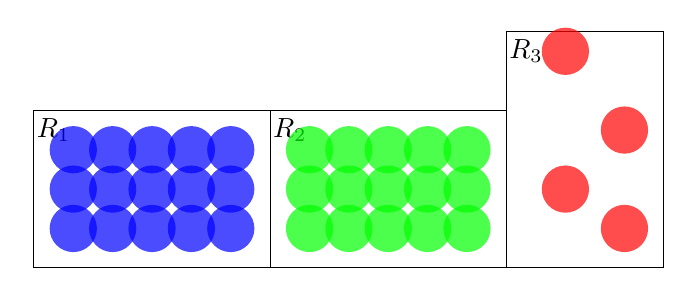
\begin{tikzpicture}[scale=0.5]

\draw  (-6,0) rectangle (-12,4);
\node at (-11.5,3.5) {$R_1$};

\draw  (0,0) rectangle (-6,4);
\node at (-5.5,3.5) {$R_2$};

\draw  (0,0) rectangle (4,6);
\node at (0.5,5.5) {$R_3$};

\def \n {5}
\def \radius {3cm}
\def \margin {8} % margin in angles, depends on the radius

\foreach \x in {0,...,4}{\foreach \y in {0,...,2}{
  \node[rfid] at (-11 + \x,3 - \y) {};
}}
\foreach \x in {0,...,4}{\foreach \y in {0,...,2}{
  \node[rfid,fill=green] at (-5 + \x,3 - \y) {};
}}

\node[rfid,fill=red] at (1.5,5.5) {};
\node[rfid,fill=red] at (3,3.5) {};
\node[rfid,fill=red] at (1.5,2) {};
\node[rfid,fill=red] at (3,1) {};

\end{tikzpicture}